\documentclass[12pt,leqno]{article}
\usepackage{polski}
\usepackage[utf8]{inputenc}
\usepackage[T1]{fontenc}
\usepackage{times}

\usepackage{amsfonts}
\usepackage{amsmath}
\usepackage{bm}
\usepackage{mathtools}
\mathtoolsset{showonlyrefs}


\usepackage{tabularx}
\usepackage{array}
\newcolumntype{Y}{>{\centering\arraybackslash}X}
\newcolumntype{Z}{>{\centering\arraybackslash}p}
\usepackage{multirow}
\usepackage{hyperref}

\usepackage{enumitem}
\usepackage{float}


\usepackage{graphicx}
\usepackage{rotating}
\usepackage{subcaption}


\usepackage{animate}

\renewcommand{\thesection}{\arabic{section}}
\renewcommand{\thesubsection}{\arabic{section}.\arabic{subsection}}
\usepackage{wrapfig}



\usepackage{amsmath}
\usepackage{amsthm}
\usepackage{dsfont}
\newtheorem{lema}{Lemma}

\newtheoremstyle{exer}{20pt}{10pt}{}{0pt}{\bfseries}{.\\}{.5em}{}
\theoremstyle{exer}
\newtheorem{ex}{Ex}

%\usepackage[a4paper,total={6in,10in}]{geometry}
\usepackage[a4paper,total={7in,10in}]{geometry}
%\newtheoremstyle{style name}{space above}{space below}{body font}{indent amount}{head font}{head punct}{after head space}{head spec}


\begin{document}
	\section{Analiza zależności między }
	Analizujemy zależność między ceną, a objętością. Przyjrzyjmy się zalezności naszych danych na wykresie.
	\begin{figure}[H]\label{fig:v_vs_price}\centering
		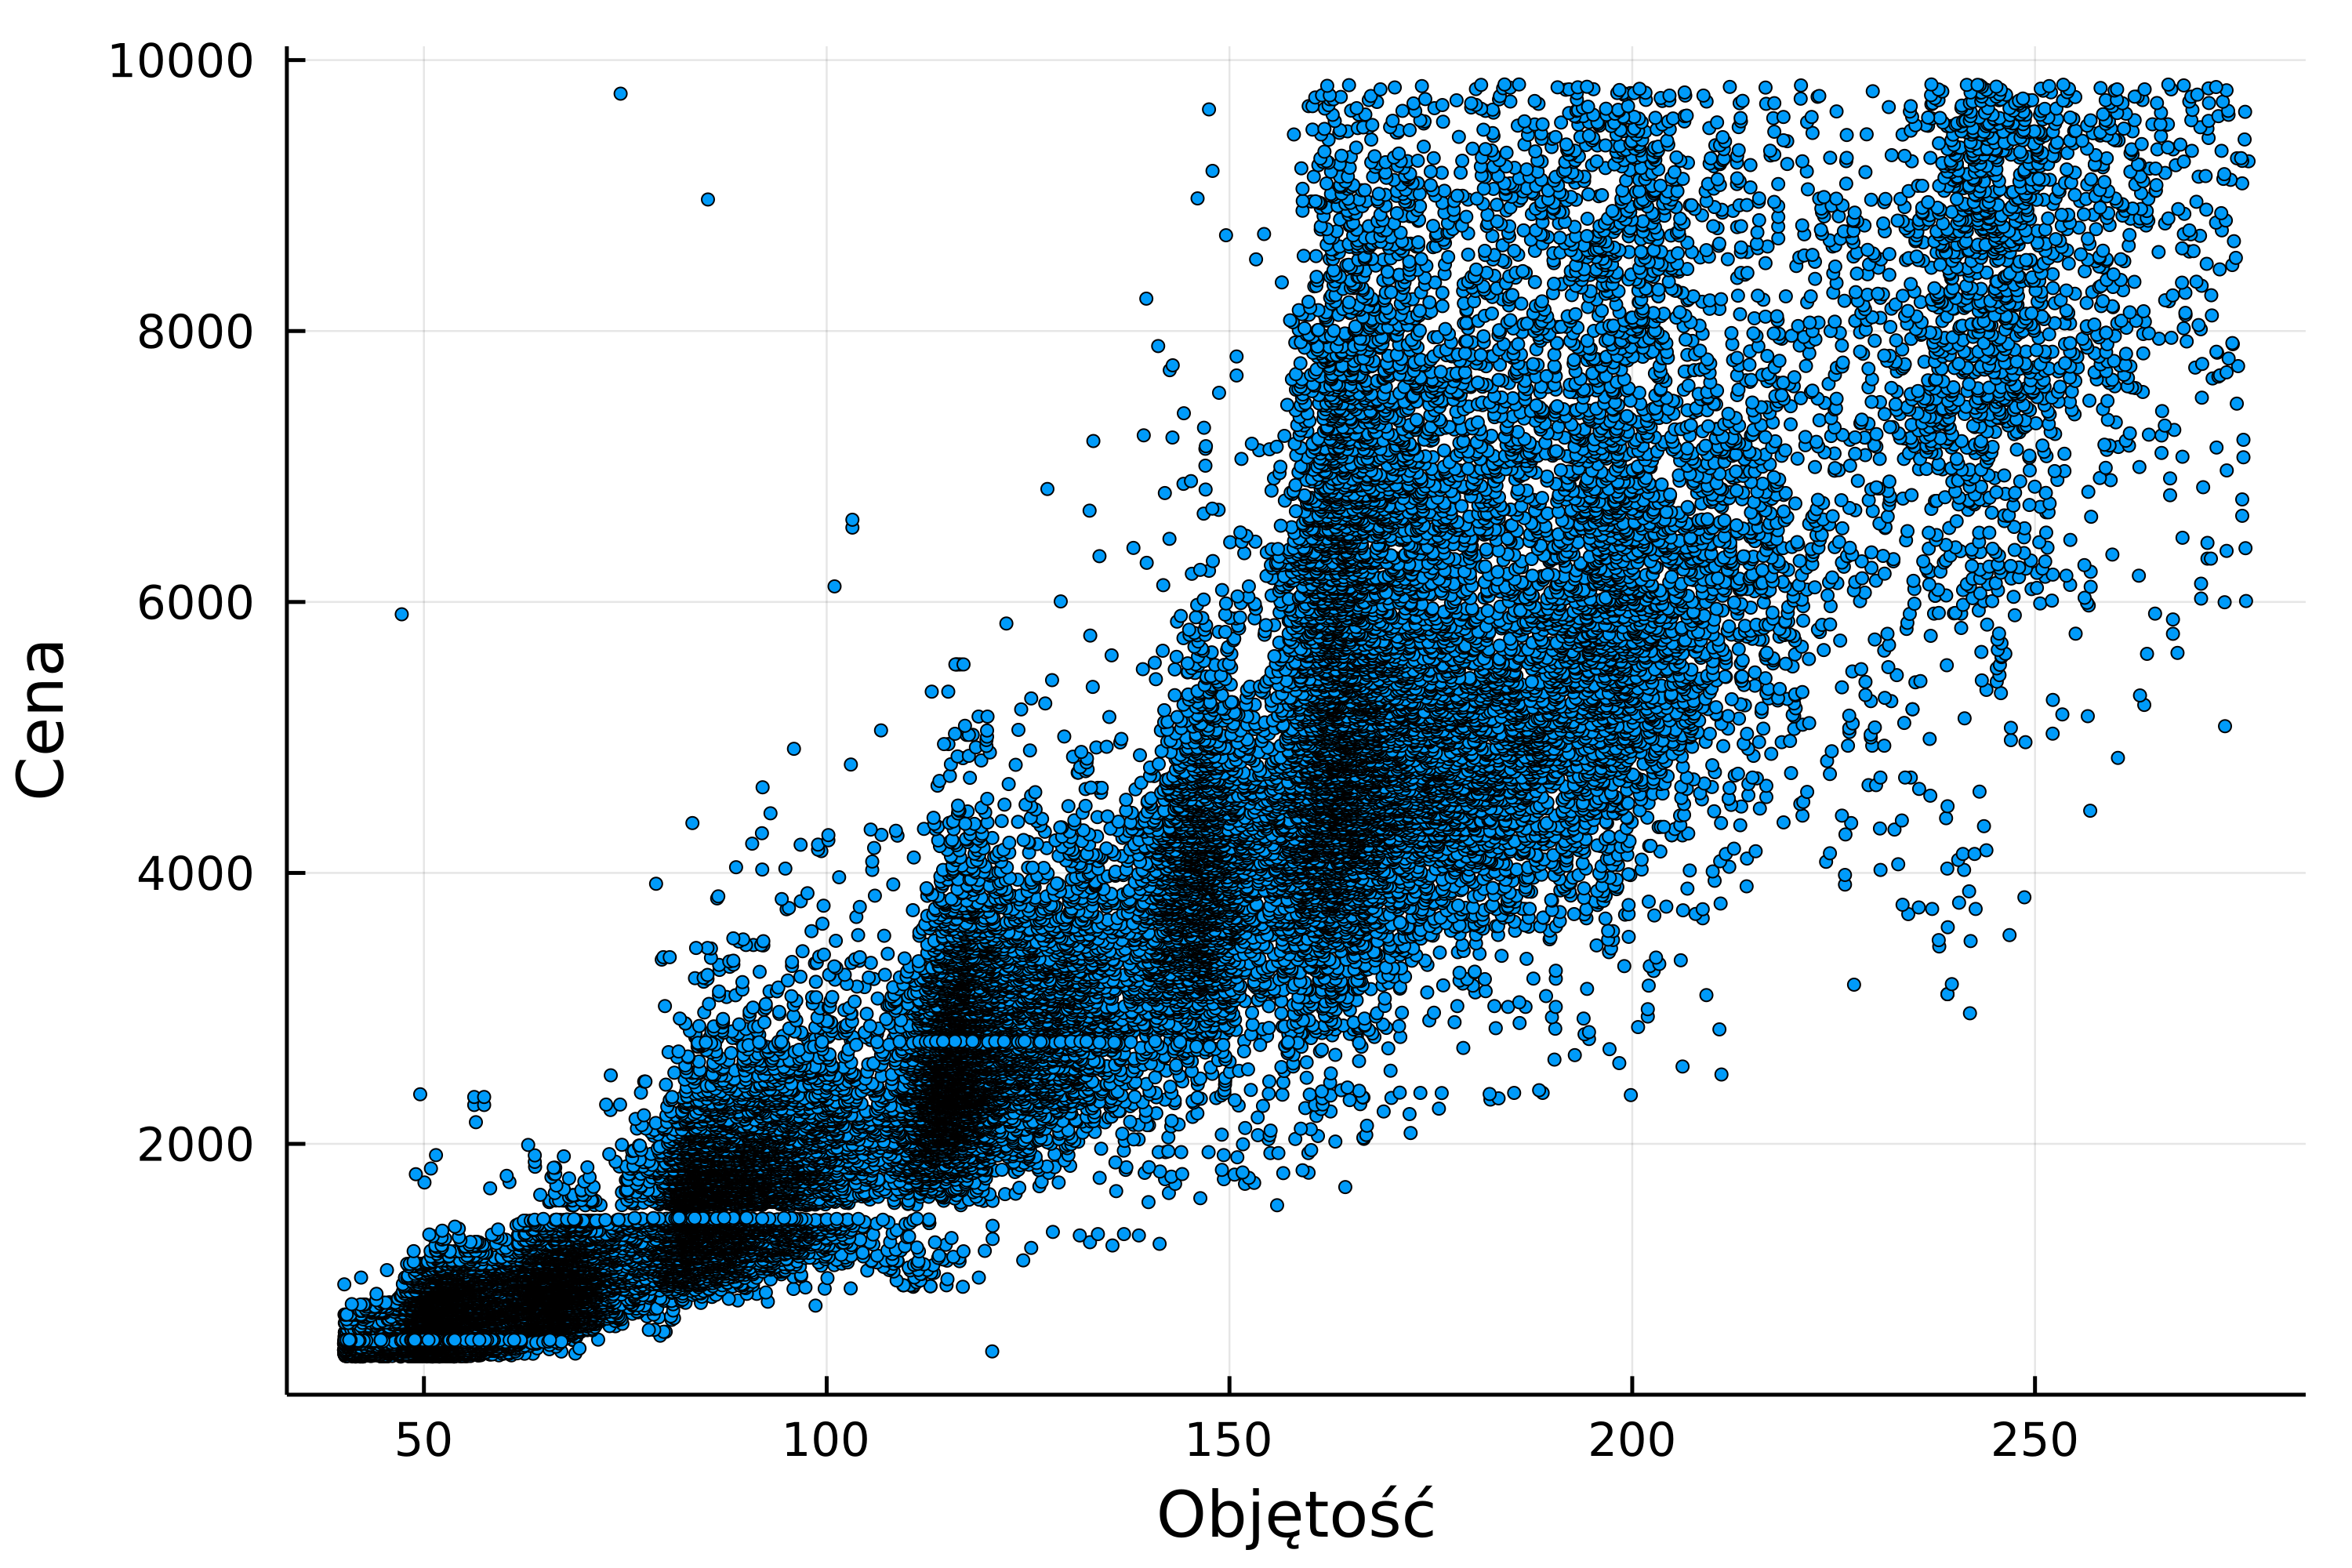
\includegraphics[width=4\columnwidth/5]{images/Budnik/v_vs_price.png}\caption{Wykres cena-objętość}
	\end{figure}
	Z wykresu możemy zauważyć silną zależność między naszymi danymi. Z powodu rozłożenia naszych danych zależność ta może być linowa. W celu określenia tej zależności obliczymy współczynnik korelacji pearsona
	\begin{equation}
		\rho=\frac{\sum_{i=1}^n\left(x_i-\overline{x}\right)\left(y_i-\overline{y}\right)}
		{\sqrt{\sum_{i=1}^n\left(x_i-\overline{x}\right)^2}\sqrt{\sum_{i=1}^n\left(y_i-\overline{y}\right)^2}}\approx0.93,
	\end{equation}
	gdzie $x_i$, $y_i$ to $i$-te obserwacje odpowiednio objętości oraz ceny, $\overline{x}$ oznacza średnią z $x$, a $n$ to rozmiar próby, oznaczeniami tymi będziemy posługiwali się w całym raporcie. Wartość ta jest blisko wartości $1$, zatem nasze dane są silnie skorelowane dodatnie oraz liniowo. Dlatego model, którym będziemy opisywać dane będzie miał postać
	\begin{equation}\label{eq:reg}
		Y_i=\beta_0+\beta_1x_i+\xi_i,
	\end{equation}
	gdzie $\xi_i$ jest losowym błędem pomiarowym. $Y_i$ jest zmienną losową, której realizacją jest zaobserwowana wartość $y_i$. Zgodnie z treścią polecenia zakładamy, że wszystkie zminne losowe $\xi_i$ są idd. oraz mają rozkład normalny ze średnią 0. Naszym zadaniem będzie estymować wartość $\hat y_i$ poprzez estymowanie realizacji zmiennych losowych $\hat \beta_0$ oraz $\hat\beta_1$.
	\subsection{Estymacja punktowa}
	By stworzyć estymator ceny $\hat y$ skorzystamy z metody najmniejszych kwadratów. Do estymacji parametrów $\beta_0$ oraz $\beta_1$, występujące we wzorze \eqref{eq:reg}, wykorzystamy losowo wybrane $80\%$ naszych danych. Pozostałe $20\%$ posłuży nam w celu sprawdzenie poprawności modelu. Estymowane parametry, w danej realizacji $Y$, mają wartość
	\begin{equation}
		\hat\beta_1=\frac{\sum_{i=1}^n\left(x_i-\overline{x}\right)\left(y_i-\overline{y}\right)}
		{\sum_{i=1}^n\left(x_i-\overline{x}\right)^2}\approx39.255 \quad \text{oraz} \quad
		\hat\beta_0=\overline{y}-\beta_1\overline{x}\approx-1564.73.
	\end{equation}
	Estymowana wartośc ceny $\hat y$ w modelu \eqref{eq:reg} będzie miała postać
	\begin{equation}
		\hat y_i = 39.255\cdot x_i -1564.73.
	\end{equation}
	\subsection{Estymacja przedziałowa}
	W tym przypadku będziemy szukać przedziału do w którym będzie należał nasz $Y_i$ z dużym prawdopodobieństwem. Będziemy chcieli by prowdopodobieństow to wynosiło $1-\alpha$. Znany jest fakt, że w modelu \eqref{eq:reg} zmienna $\hat{Y}_i$ ma poniższe parametry
	\begin{equation}
		\mathbb{E}\hat Y_i = \beta_0+\beta_1x_i \quad\text{oraz}\quad Var \hat Y_i=Var\left(\xi_1\right)\left(\frac{1}{n}+\frac{(x_0-\overline{x})}{\sum_{i=1}^{n}\left(x_i-\overline{x}\right)^2}\right).
	\end{equation} 
	Jeśli $Var\left(\xi_1\right)$ nie jest znana w jej miejsce wstawiamy jej estymator
	\begin{equation}
		s^2=\frac{1}{n-2}\sum_{i=1}^{n}\left(Y_i-\hat Y_i\right)
	\end{equation}
	otrzymując estymator $Var \hat Y_i$ i wtym przypadku zmienna losowa
	\begin{equation}
		\frac{\hat Y_i-\mathbb{E}\hat Y_i}{s^2\left(\frac{1}{n}+\frac{(x_0-\overline{x})}{\sum_{i=1}^{n}\left(x_i-\overline{x}\right)^2}\right)}
	\end{equation}
	ma rozkład t-studenta z $n-2$ stopniami swobody. Niech $z_{\alpha/2}$ będzie $1-\alpha/2$ kwantylem z tego rozkładu. Wtedy możemy napisać, że 
	\begin{equation}
		\mathbb{P}\left(\hat Y_0 - z_{\alpha/2}s\sqrt{\frac{1}{n}+\frac{\left(x_0-\overline{x}\right)^2}{\sum_{i=1}^n\left(x_i-\overline{x}\right)^2}}\leq Y_0\leq\hat Y_0 + z_{\alpha/2}s\sqrt{\frac{1}{n}+\frac{\left(x_0-\overline{x}\right)^2}{\sum_{i=1}^n\left(x_i-\overline{x}\right)^2}}\right)=1-\alpha.
	\end{equation}
	Zatem naszymi przedziałami ufności dla danej realizacji $Y$ będzie 



\end{document}